\begin{frame}
\frametitle{Interactive Multisensor Snow and Ice Mapping System}
\begin{columns}

\column{0.5\textwidth}

\begin{itemize}
    \item Daily snow/ice coverage. 
    \item Matrix style output on FTP site
    \item Current tools for visualization
\end{itemize}

\begin{figure}
    \centering
    \begin{minipage}{.85\columnwidth}
    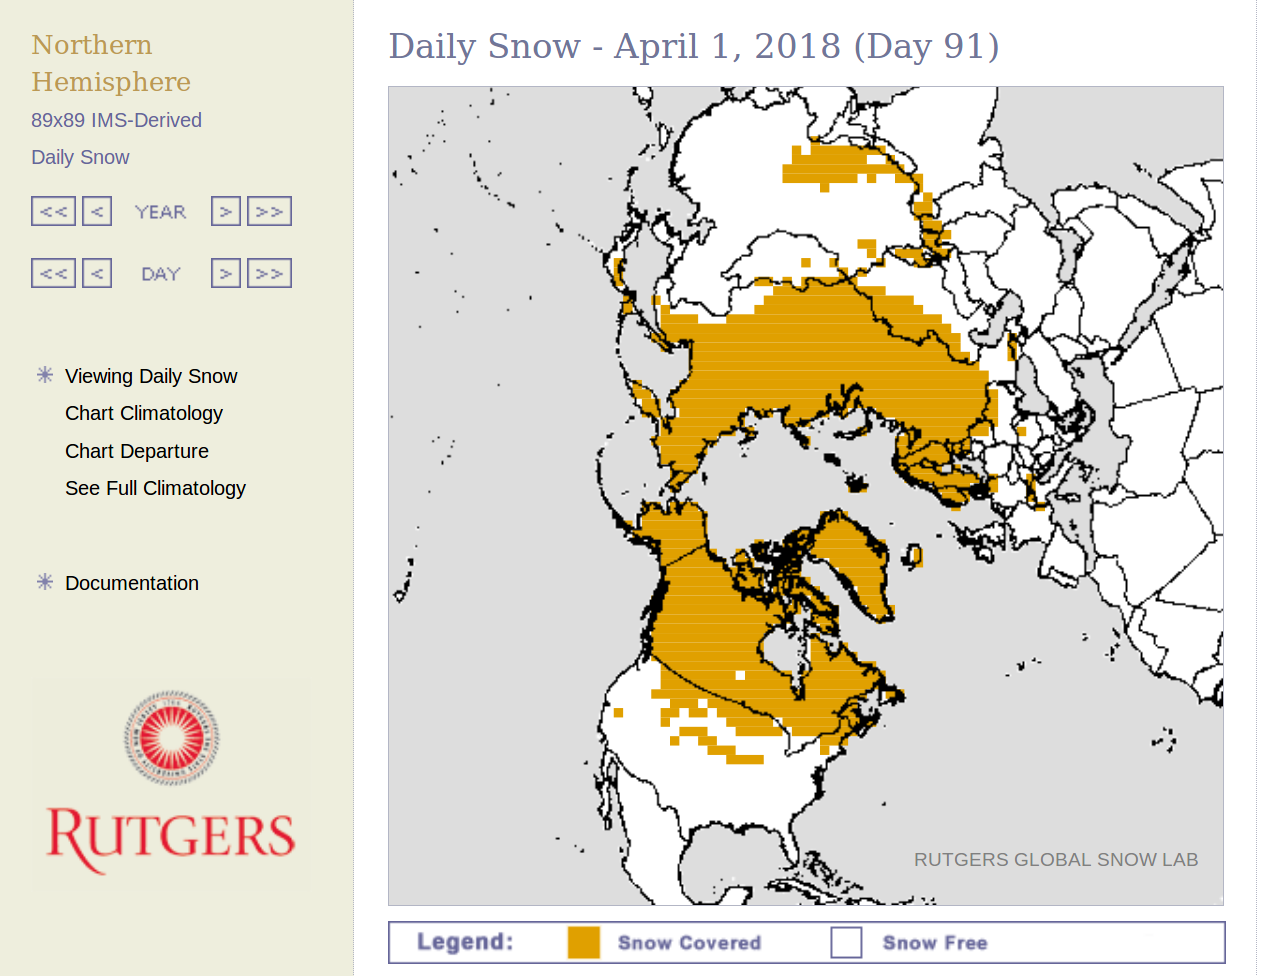
\includegraphics[width=\linewidth]{rutgers.png}
    \caption{\tiny{IMS snow cover, \url{https://climate.rutgers.edu/snowcover/}}}
    \end{minipage}
\end{figure}

\column{0.5\textwidth}

\begin{figure}
    \centering
    \begin{minipage}{.75\columnwidth}
    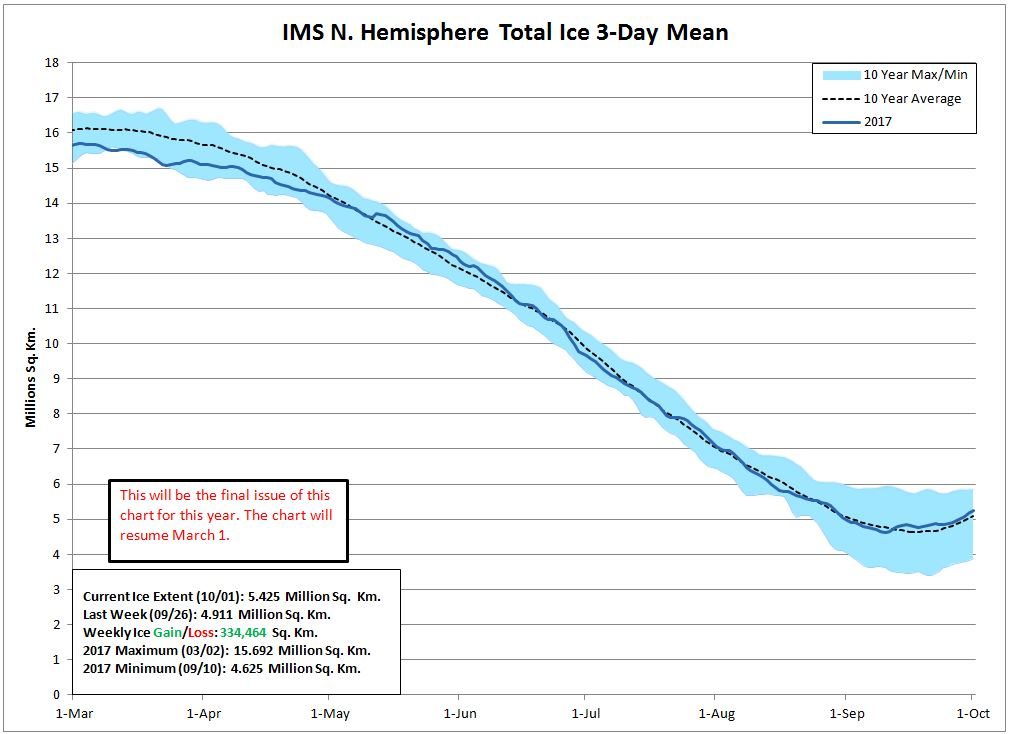
\includegraphics[width=\linewidth]{ims_data.jpg}
    \caption{\tiny{IMS snow area, \url{http://www.natice.noaa.gov/ims/}}}
    \end{minipage}
\end{figure}
\vspace*{-.5cm}
\underline{\textbf{Research topics}}
\begin{itemize}
    \item Calculate grid area?
    \item Estimate snow/ice coverage in $km^2$
    \item Estimated error vs other products?
\end{itemize}
\end{columns}
\end{frame}

\begin{frame}
\frametitle{Introducing IMS - Tibet Snow Man}
\begin{columns}
\column{0.5\textwidth}
\begin{figure}
\vspace*{-1.25cm}
    \centering
    \begin{minipage}{.85\columnwidth}
    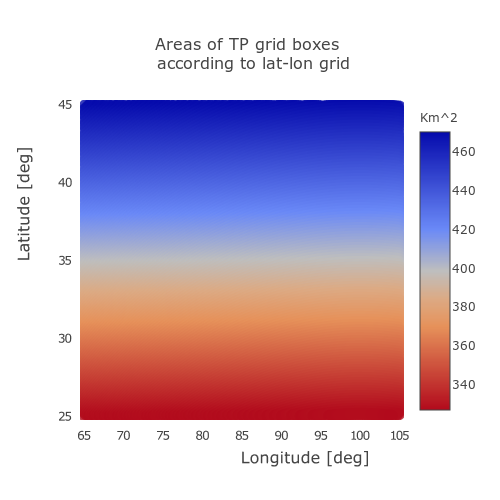
\includegraphics[width=\linewidth]{areas_of_tibet_grid_i.png}
    \caption{\tiny{Time series comparison between 24 x 24km 2 assumption and area calcu-
lation via shoe-lace formula.}}
    \end{minipage}
\end{figure}

\column{0.5\textwidth}
\begin{figure}
    \centering
    \begin{minipage}{.95\columnwidth}
    %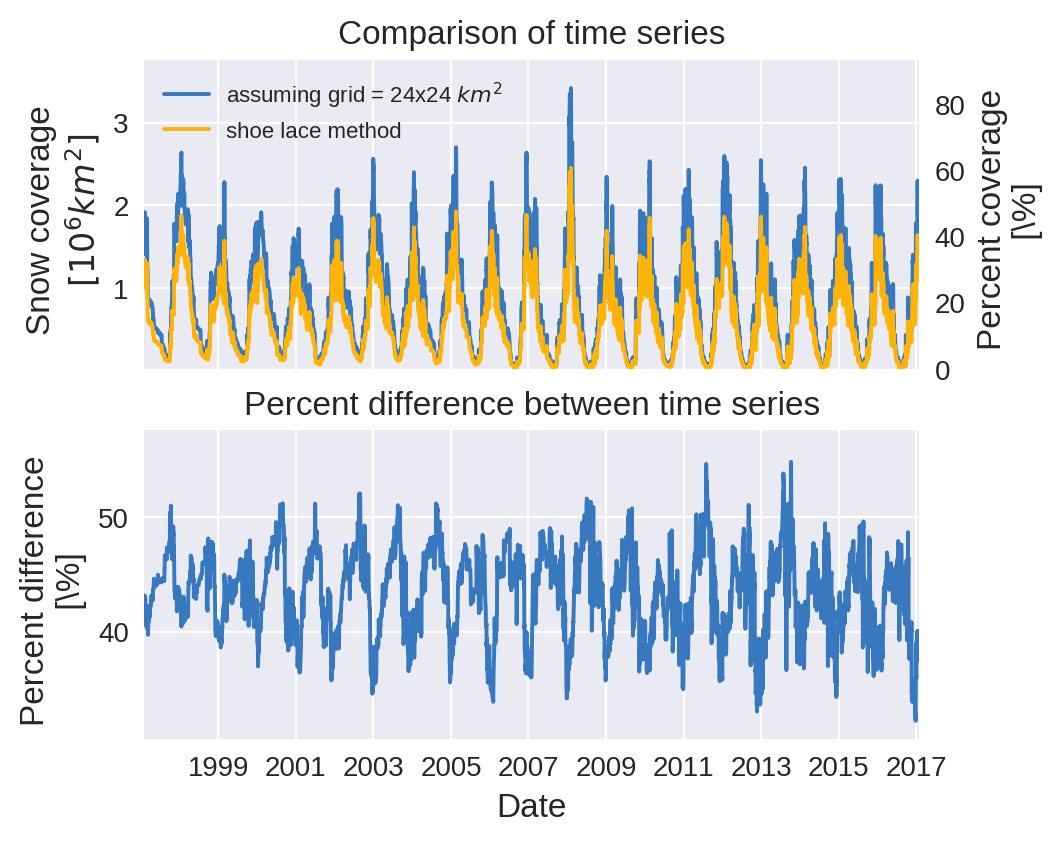
\includegraphics[width=\linewidth]{ts-compare.png}
    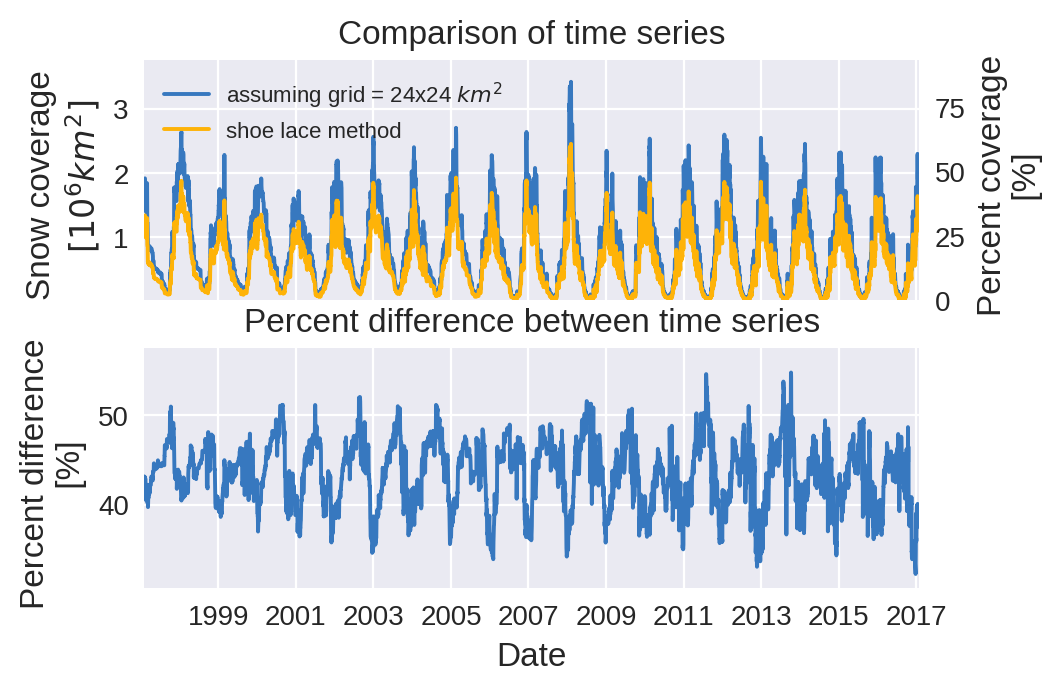
\includegraphics[width=\linewidth]{assumption.png}
    \caption{\tiny{Time series comparison between $24 x 24km^2$ assumption and area
calculation via shoe-lace formula.}}
    \end{minipage}
\end{figure}
\end{columns}
\end{frame}

\begin{frame}
\frametitle{Introducing IMS - Tibet Snow Man}
\begin{figure}
    \centering
    \begin{minipage}{.9\columnwidth}
    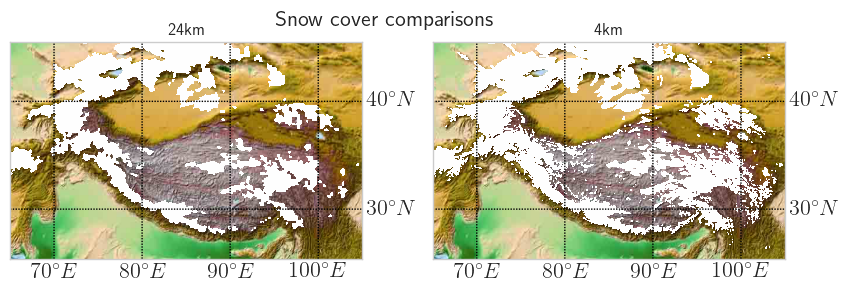
\includegraphics[width=\linewidth]{tibet-snow-res-compare.png}
    \caption{\tiny{Time series comparison between 24 x 24km 2 assumption and area calculation via shoe-lace formula. Time lapse is available at \url{https://www.youtube.com/watch?v=Kz82dwMKnLY&t=0s}}}
    \end{minipage}
\end{figure}
\end{frame}

\begin{frame}
\frametitle{Describing the Data}
\begin{columns}
\column{0.40\textwidth}
\begin{figure}
\vspace*{-.6cm}
\begin{minipage}{1\columnwidth}
\centering
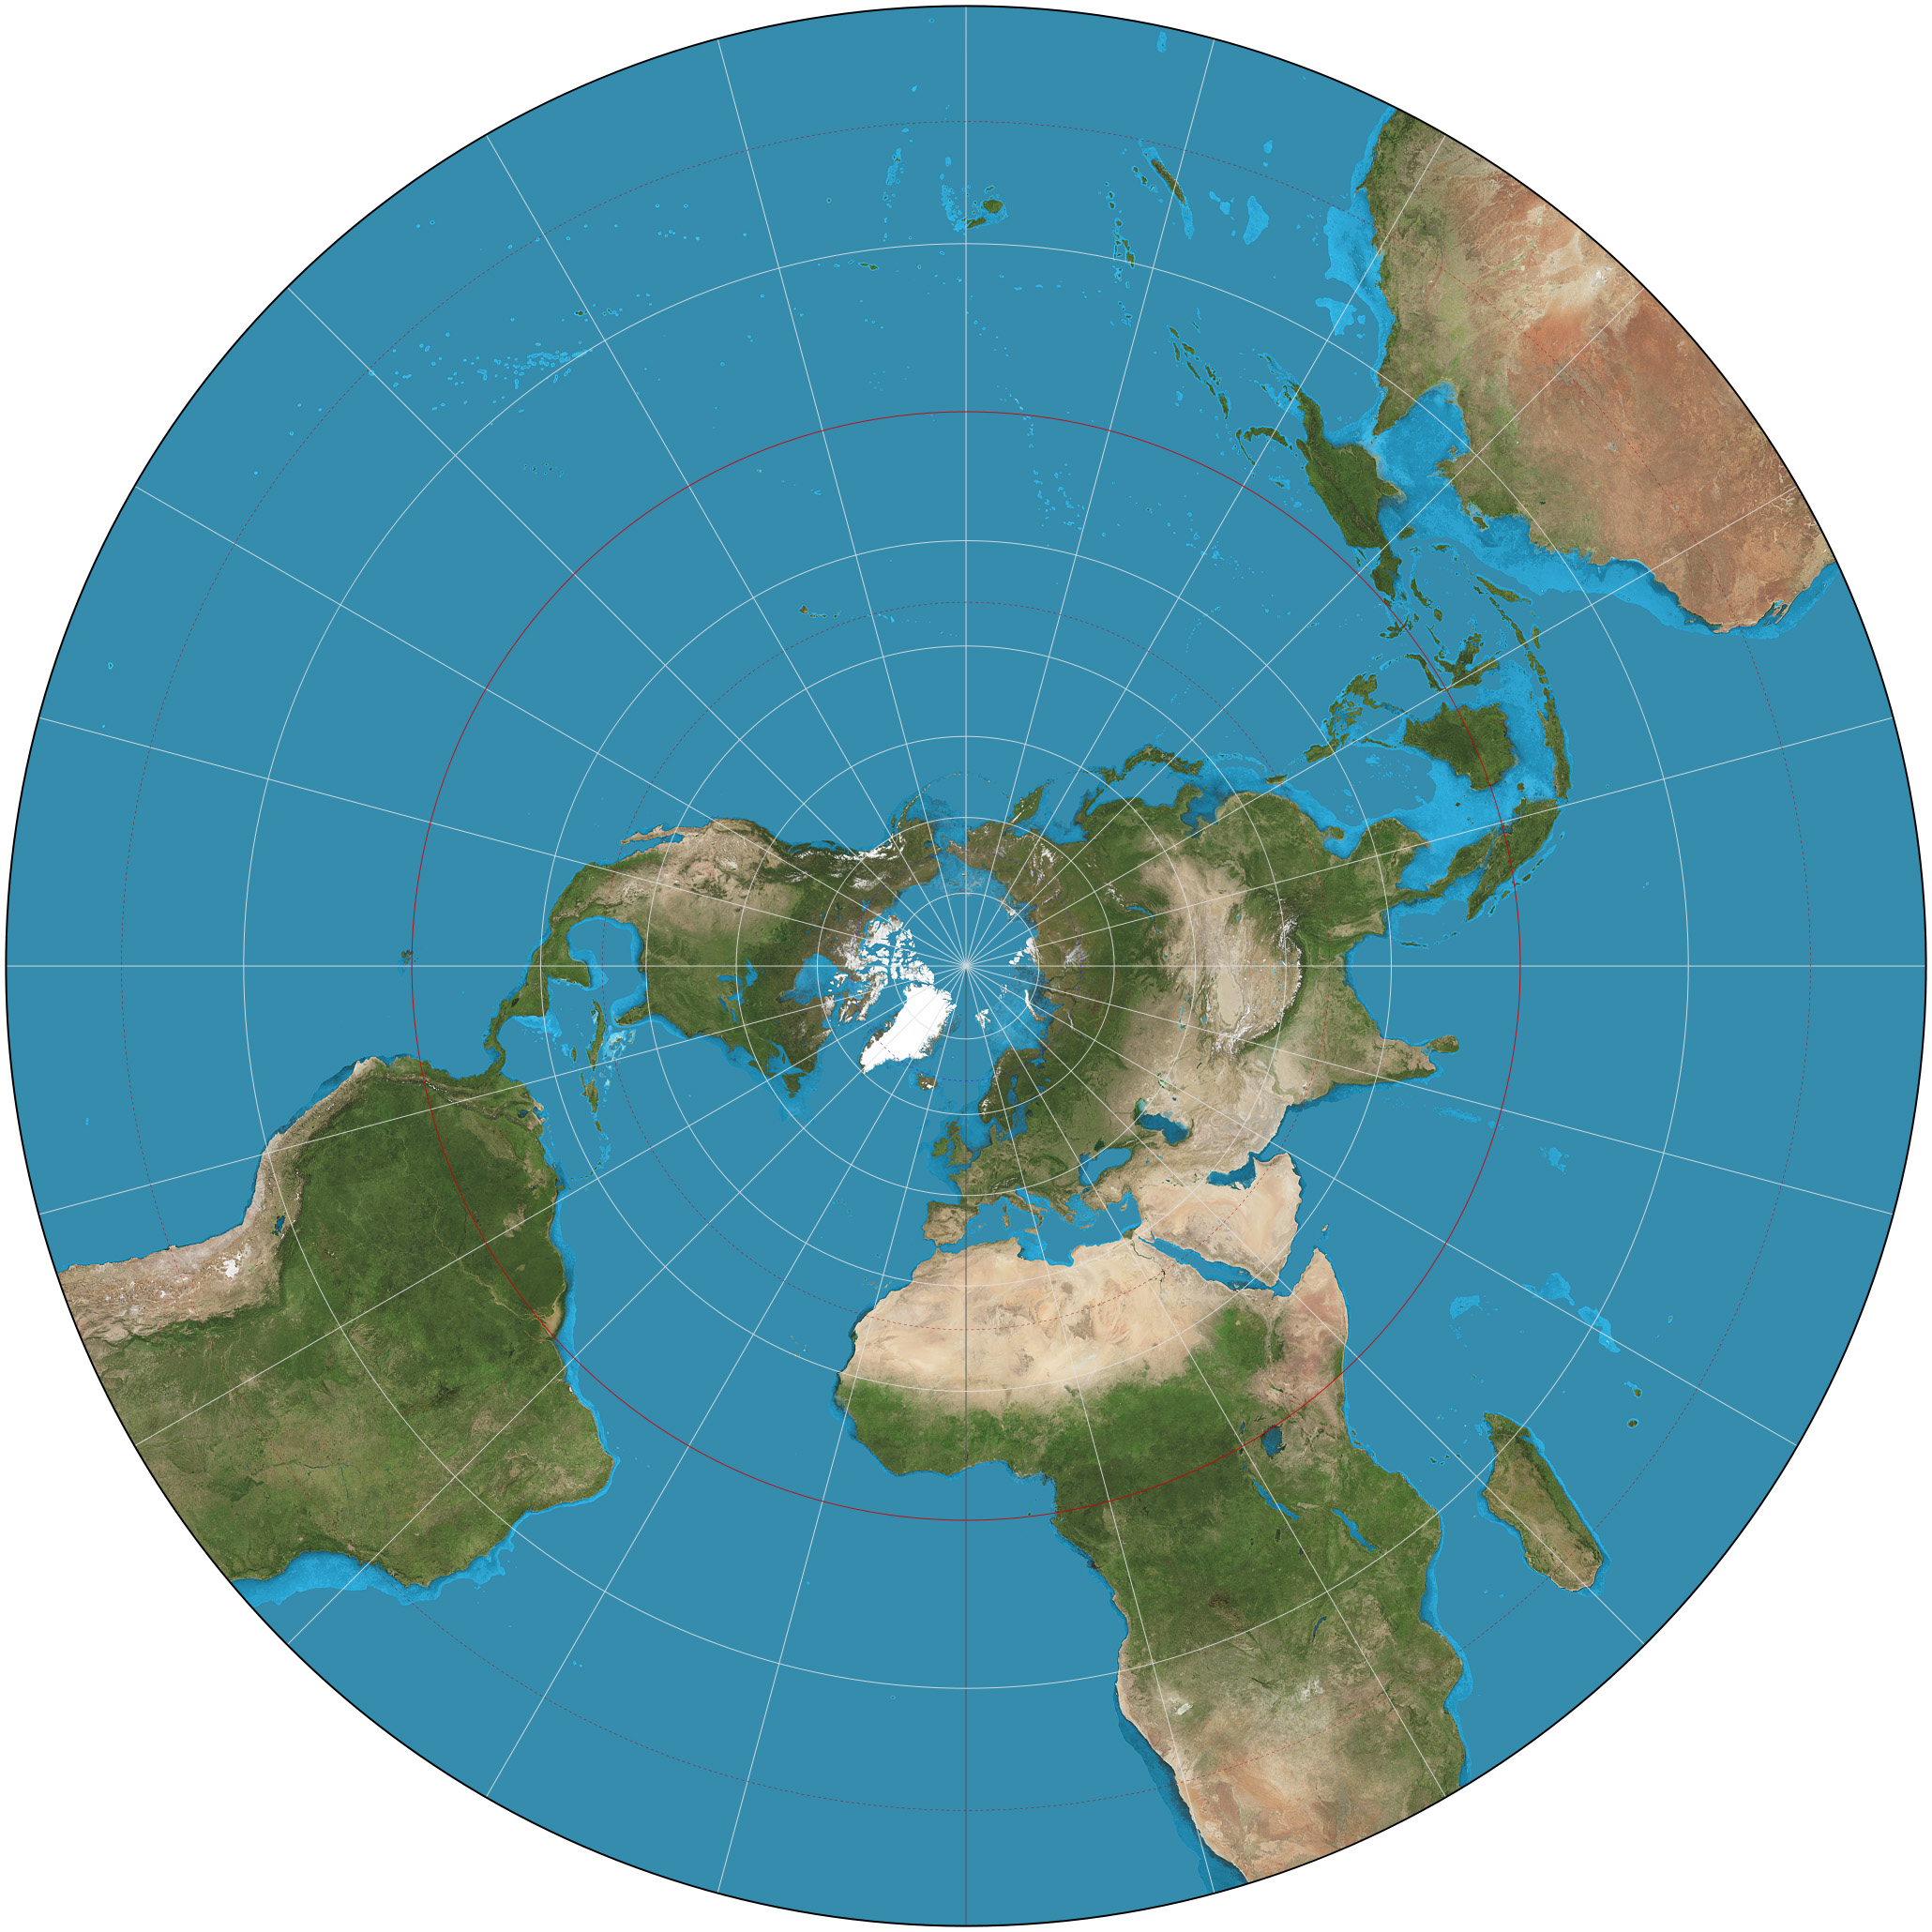
\includegraphics[width=1\linewidth]{stereographic_proj.JPG}
\caption{\tiny{Stereographic projection. Taken from \url{https://en.wikipedia.org/wiki/Stereographic_projection}}}
\end{minipage}
\end{figure}
\column{0.4\textwidth}
\begin{block}{Stereographic Projection}
Equations to map a sphere point $(\phi, \lambda)$ to a Cartesian point $(x,y)$  are below:
\begin{equation*}
x = 2R \ k_0 \tan (\frac{\pi}{4} - \frac{\phi}{2}) \sin (\lambda - \lambda_{0} )
\end{equation*}
\begin{equation*}
y = -2R \ k_0 \tan (\frac{\pi}{4} - \frac{\phi}{2})\cos(\lambda - \lambda_{0})
\end{equation*}
The length scale factor $k$ is
\begin{equation*}
k = \frac{2k_{0}}{1+\sin(\phi)},
\end{equation*}
and $(\phi_0,\lambda_0)$ is a designated center point.
\end{block}
\end{columns}
\end{frame}

\begin{frame}
\frametitle{Describing the Data}
\begin{columns}
\column{0.45\textwidth}
\begin{figure}
\vspace*{-.6cm}
\begin{minipage}{1\linewidth}
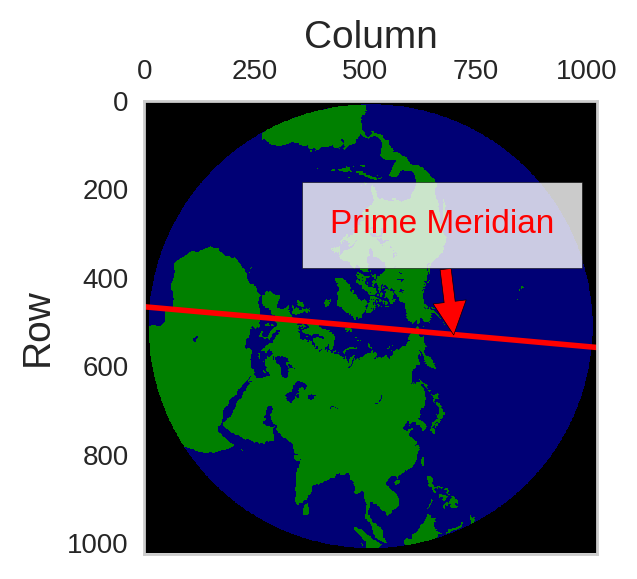
\includegraphics[width=\linewidth]{dry_planet_24km.png}
\caption{\tiny{Grid coordinate ticks of NH without snow
and ice cover. IMS provides daily files in an n x n for-
mat. The data is given in .asc files but mirrored to the
figure shown. The file represents a stereographic projec-
tion, with the 80$^\circ$ meridian line pointing up. IMS rotates
the prime meridian by about 10.22$^\circ$ clockwise to the hori-
zontal. This figure shows the 24km resolution data, which
has n = 1024.}}
\end{minipage}
\end{figure}
\column{0.45\textwidth}
\begin{figure}
\begin{minipage}{1\linewidth}
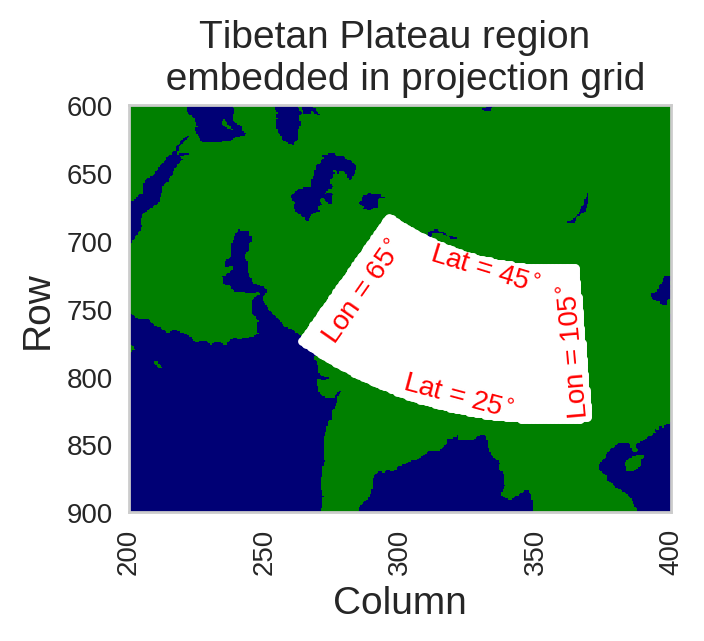
\includegraphics[width=\linewidth]{zoomed_earth.png}
\caption{\tiny{The TP region (25$^\circ$ - 45$^\circ$ N and 65$^\circ$ - 105$^\circ$ E) shown
bounded in white is shown on a stereographic projection.}}
\end{minipage}
\end{figure}
\end{columns}
\end{frame}

\begin{frame}
\frametitle{Describing the Data}
\begin{columns}
\column{0.5\textwidth}
\begin{itemize}
    \item IMS claims a 24x24, 4x4, and 1x1 km resolution products. In reality, this is true at about 60$^\circ$ latitudes.
    \item IMS is a non-uniform grid.
    \item Data is coarser at the pole!
    \item Areas along latitude vary by almost x2
    \item Why make equator data finer for a snow/ice product?
    \item What are the consequences calculating snow/ice coverage with a uniform grid assumption?
\end{itemize}

\column{0.45\textwidth}
\begin{figure}[ht]
\vspace*{-.5cm}
\centering
\begin{minipage}{1\linewidth}
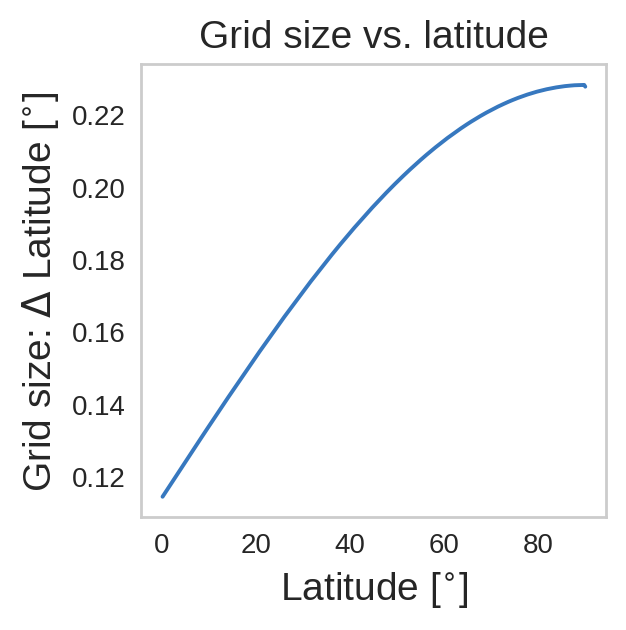
\includegraphics[width=\linewidth]{lat_diff_vs_lat.png}
\caption{\tiny{Latitude was taken from IMS latitude file: rows 0 to 512, column 512, points plotted lie approximately at $80^{\circ}E$. Grid points are distributed densely near the equator, with latitude grid spacing of $.11^{\circ}$ at the equator. The latitude grid spacing increases to $.23^{\circ}$ at the north pole.}}
\end{minipage}
\end{figure}
\end{columns}
\end{frame}

\begin{frame}
\frametitle{Describing the Data}
\begin{columns}
\column{0.45\textwidth}
\begin{figure}
\centering
\vspace*{-.6cm}
\begin{minipage}{1\linewidth}
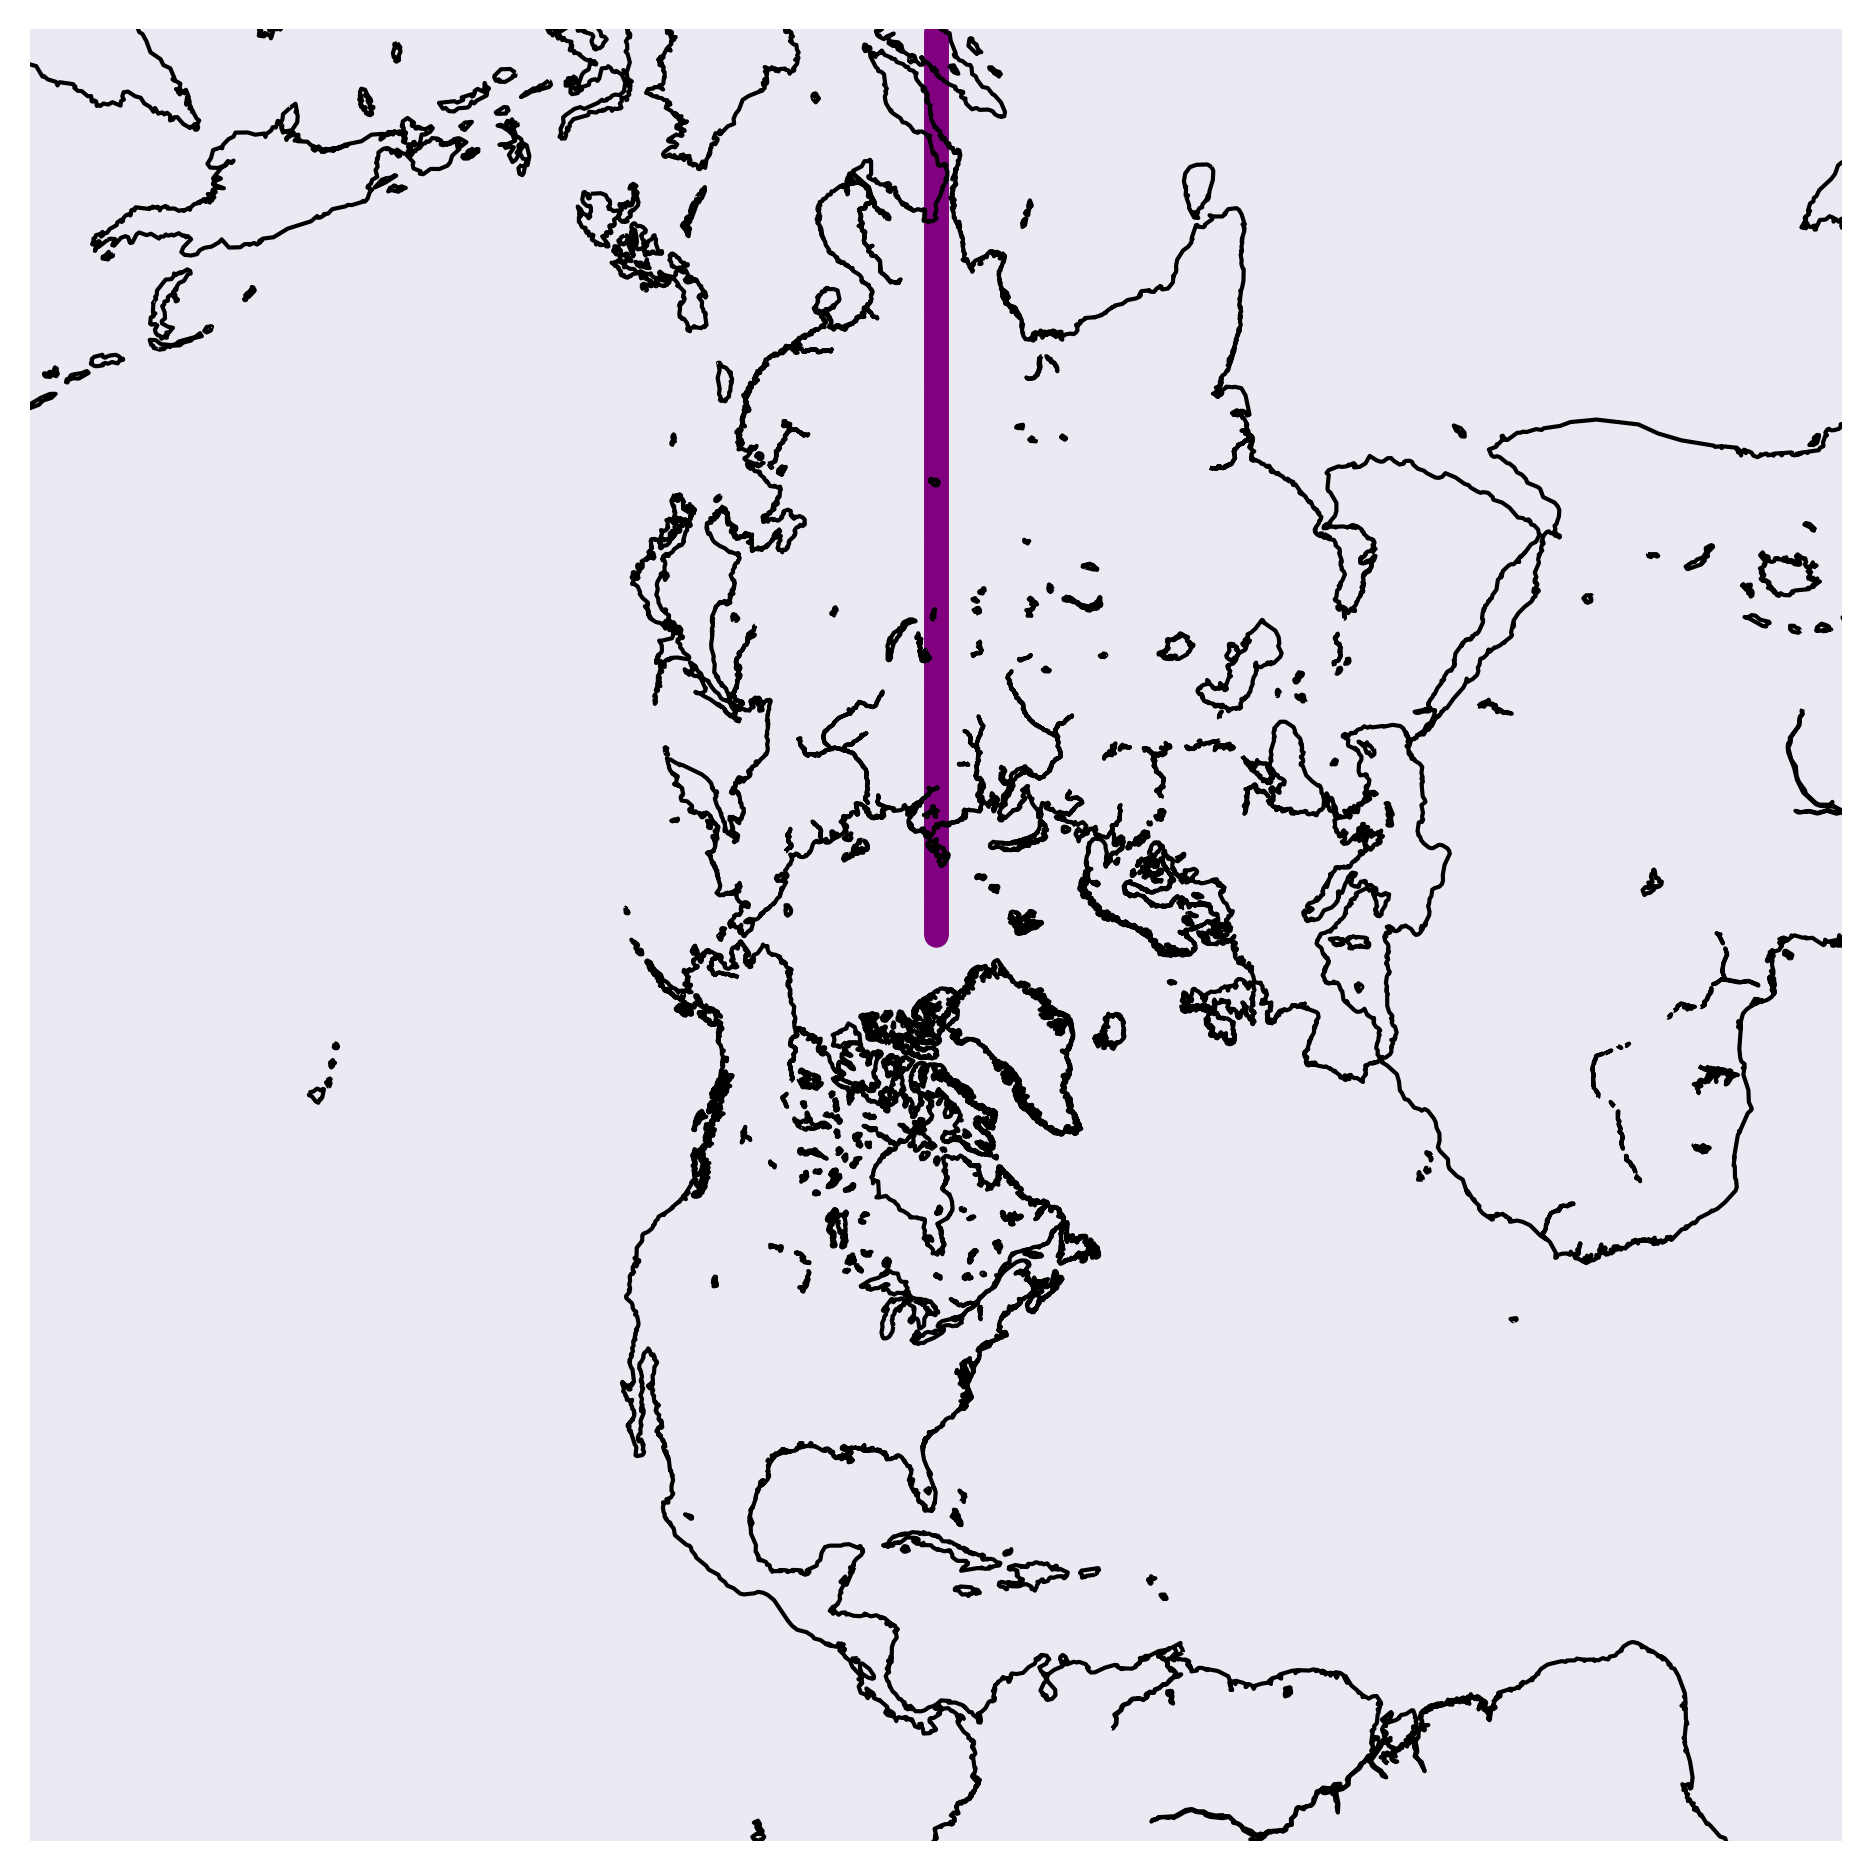
\includegraphics[width=\linewidth]{ims_line.png}
\caption{\tiny{Latitude was taken from IMS latitude file: rows 0 to 512, column 512, points plotted lie approximately at $80^{\circ}E$. }}\end{minipage}
\end{figure}

\column{0.45\textwidth}
\begin{figure}
\centering
\begin{minipage}{1\linewidth}
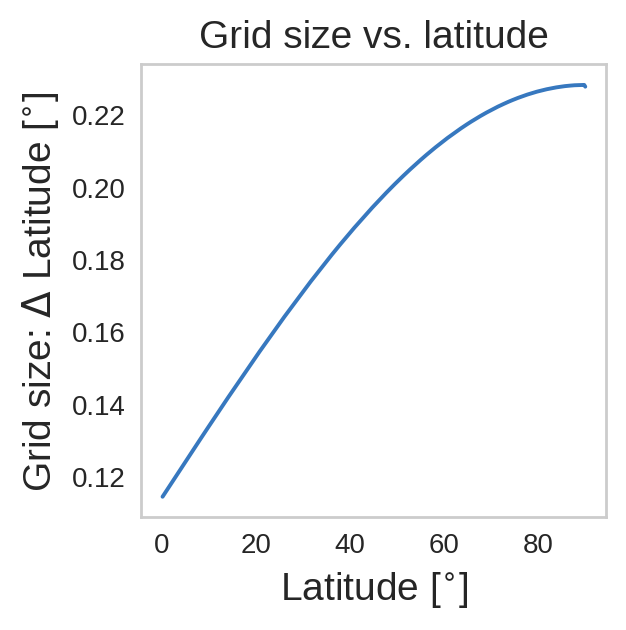
\includegraphics[width=\linewidth]{lat_diff_vs_lat.png}
\caption{\tiny{Grid points are distributed densely near the equator, with latitude grid spacing of $.11^{\circ}$ at the equator. The latitude grid spacing increases to $.23^{\circ}$ at the north pole.}}
\end{minipage}
\end{figure}

\end{columns}
\end{frame}

\begin{frame}
\frametitle{Calculating Areas}
\begin{columns}
\column{0.5\textwidth}
\begin{itemize}
    \item Question: Given a latitude-longitude grid, how can we estimate areas?
    \item Answer: Assume each point is a center of a 4-point polygon on a 2d equal-area projection. We can estimate the corners and find the areas of each cell using Green's theorem.
\end{itemize}

\column{0.45\textwidth}
\begin{figure}[ht]
\vspace*{-.5cm}
\centering
\begin{minipage}{1\linewidth}
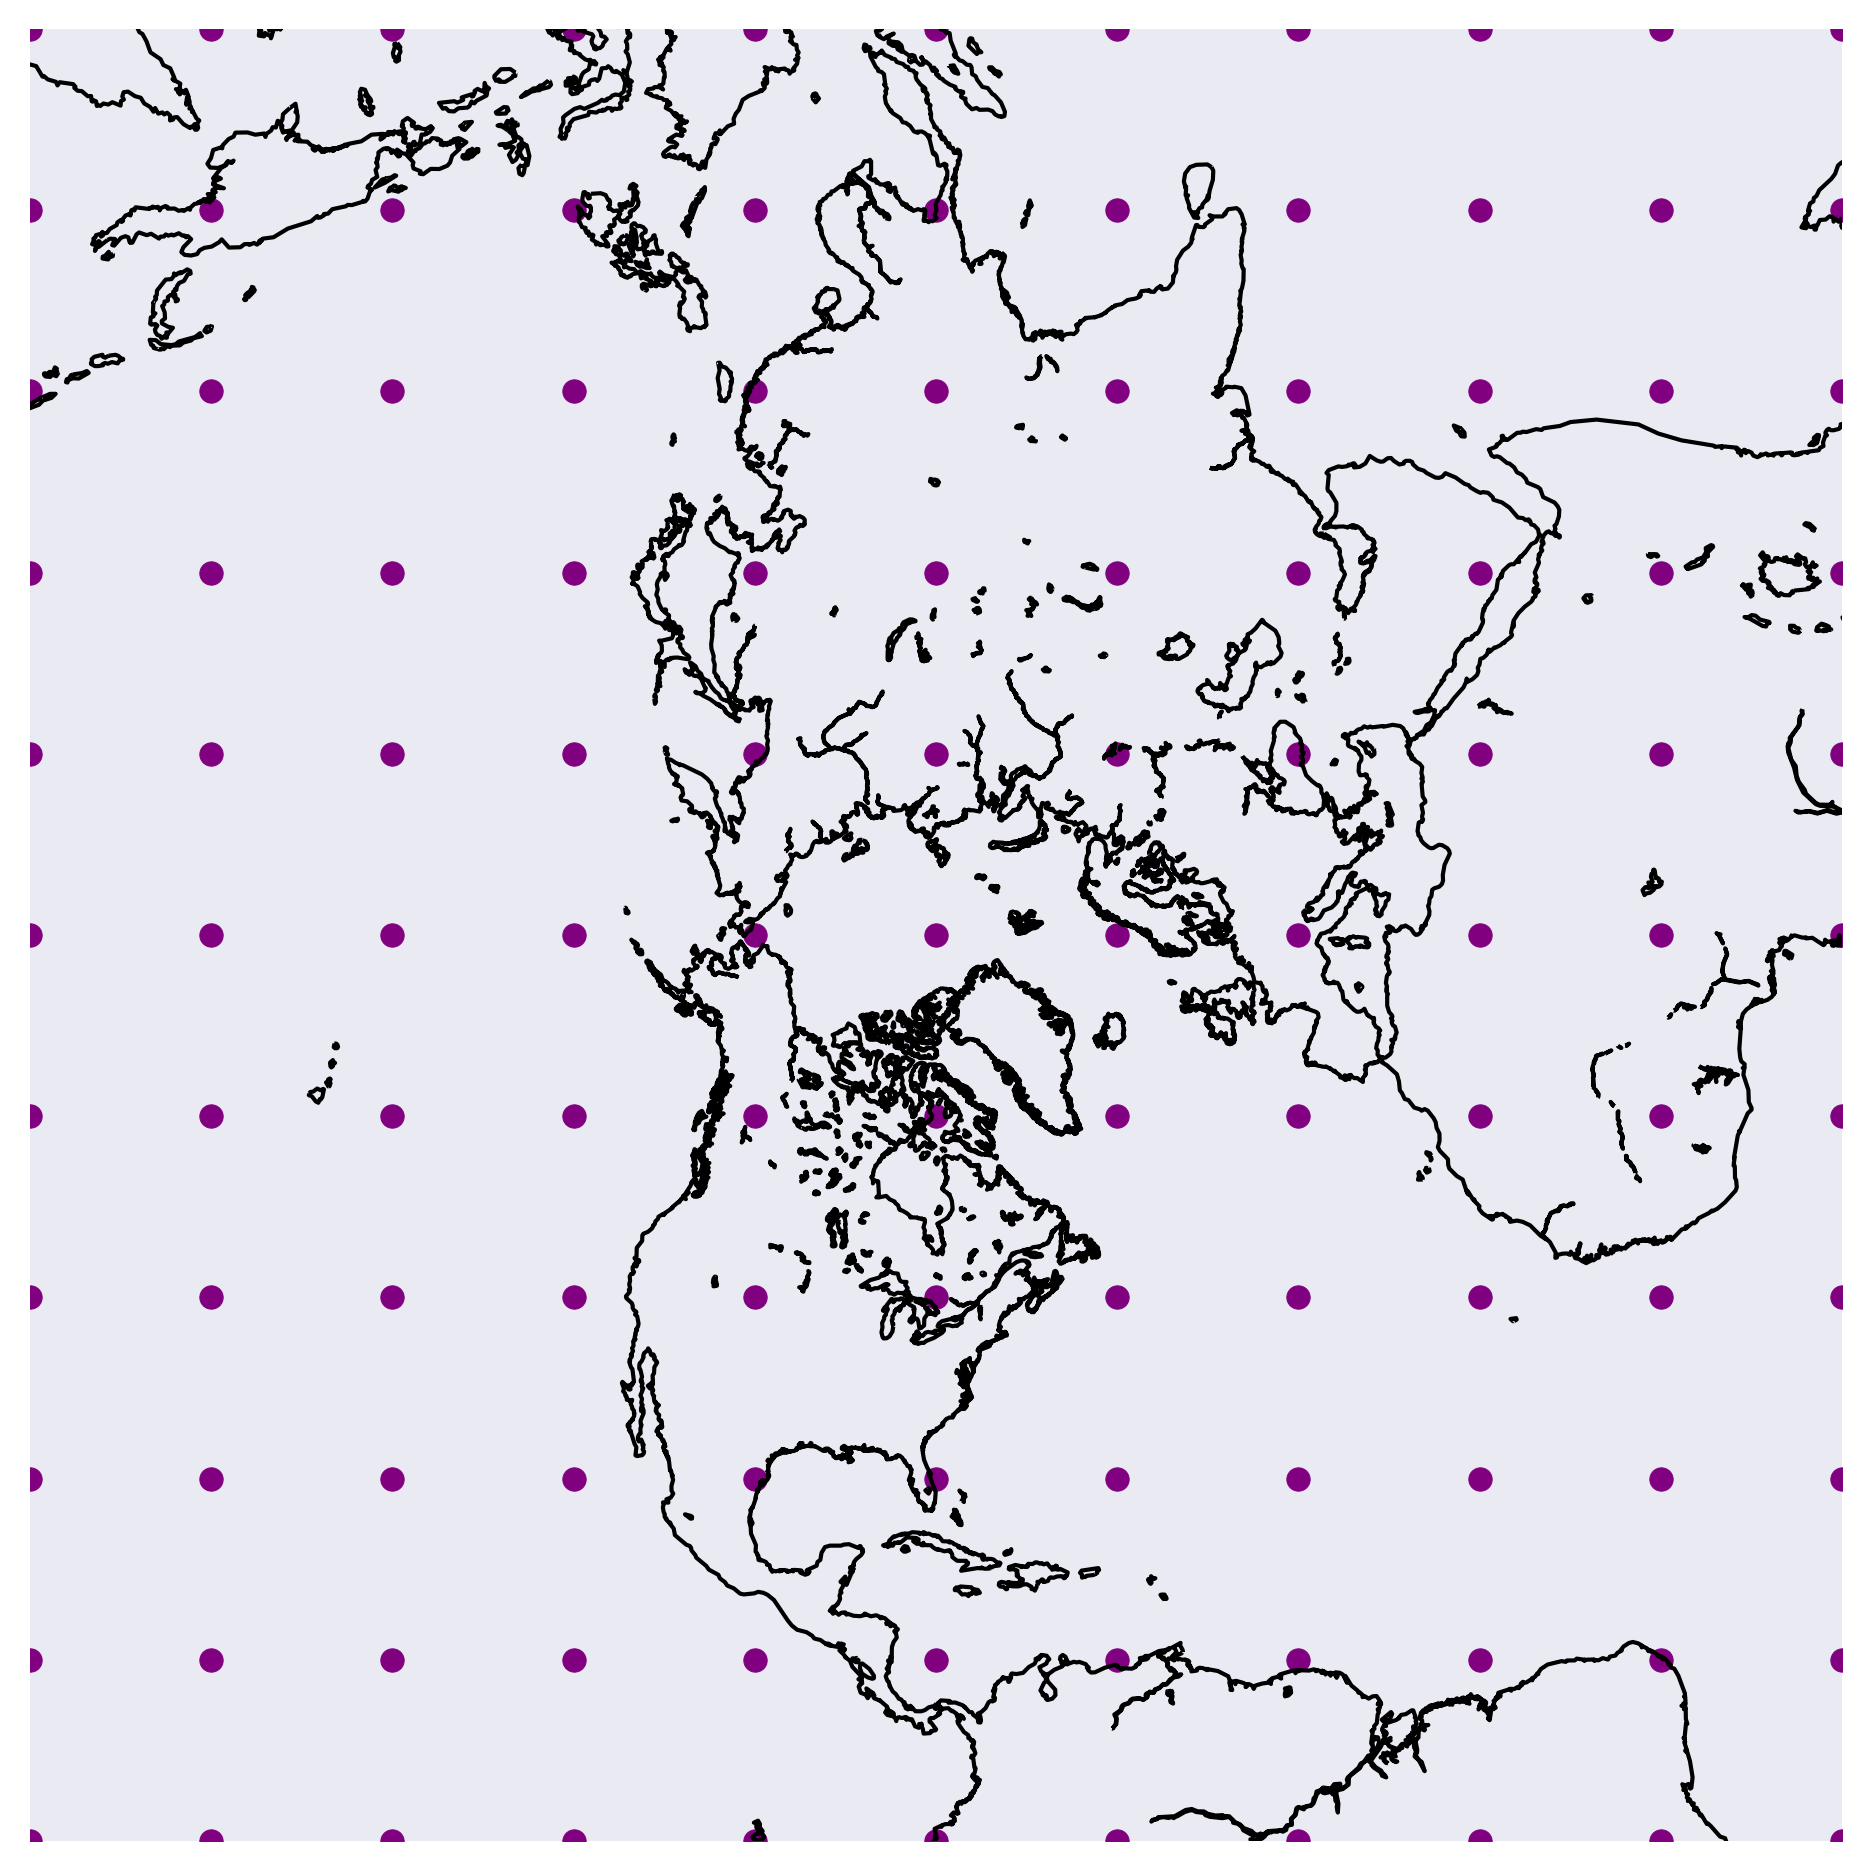
\includegraphics[width=\linewidth]{sample_grid.png}
\caption{\tiny{Sample grid}}
\end{minipage}
\end{figure}
\end{columns}
\end{frame}

\begin{frame}
\frametitle{Calculating Areas: Use an Equal Area Projection}
\begin{columns}
\column{0.40\textwidth}
\begin{figure}
\vspace*{-.6cm}
\begin{minipage}{1\columnwidth}
\centering
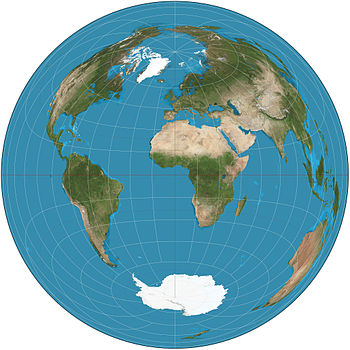
\includegraphics[width=1\linewidth]{laep.jpg}
\caption{\tiny{Lambert azimuthal equal area projection. Taken from \url{https://en.wikipedia.org/wiki/Lambert_azimuthal_equal-area_projection}}}
\end{minipage}
\end{figure}
\column{0.6\textwidth}
\begin{block}{Lambert Azimuthal Equal Area Projection}
Equations to map a sphere point $(\phi, \lambda)$ to a Cartesian point $(x,y)$  are below:
\begin{equation*}
x = R k' \cos\phi_{1}\sin(\lambda - \lambda_0)
\end{equation*}
\begin{equation*}
y = R k'[\cos\phi_{1}\sin\phi - \sin\phi_{1}\cos\phi \cos(\lambda - \lambda_{0})]
\end{equation*}
\begin{equation*}
k' = \frac{\sqrt{2}}{\sqrt{1+\sin\phi_{1}\sin\phi + \cos\phi_{1}\cos\phi \cos(\lambda\lambda_{0})}}
\end{equation*}
Where $R=6,371 km$ is the Earth's radius. For the TP, $\phi_{1} = 35^{\circ}$, $\lambda_{0}=85^{\circ}$ 
\end{block}
\end{columns}
\end{frame}

\begin{frame}
\frametitle{Calculating Areas: Estimate Grid Cell Area}
\begin{columns}
\column{0.40\textwidth}
\begin{figure}[ht]
\centering
\begin{minipage}{1\columnwidth}
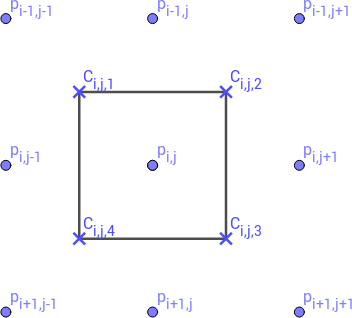
\includegraphics[width=\linewidth]{centroid_grid_w_box_cropped.png}
\caption{Grid box showing grid box corners $C_{i,j,k}$ for lat-lon point $p_{i,j}$ calculated using shoe-lace formula.}
\end{minipage}
\end{figure}
\column{0.55\textwidth}
\begin{block}{Corner/Centroids}
A grid point $p_{i,j}$ has four corners $C_{i,j,k}$. Corners are the centroids of the bounding square.
\begin{align*}
C_ij1 &= \frac{1}{4}( p_{i-1,j-1}+ p_{i,j-1}+ p_{i,j} + p_{i-1,j} ) \\
C_ij2 &= \frac{1}{4}( p_{i-1,j}+ p_{i-1,j+1} + p_{i,j+1}+ p_{i,j} ) \\
C_ij3 &= \frac{1}{4}( p_{i,j}+ p_{i,j+1} + p_{i+1,j+1}+ p_{i+1,j} ) \\
C_ij4 &= \frac{1}{4}( p_{i-1,j}+ p_{i,j} + p_{i+1,j} + p_{i-1,j+1} )
\end{align*}
\end{block}
\end{columns}
\end{frame}

\begin{frame}
\frametitle{Calculating Areas: Estimate Grid Cell Area}
\begin{block}{Shoelace/Surveyor's Formula}
Discreet Green's Theorm estimates area on a 2D surface. Given a set of vectors $x_k$, $y_k$ of the four corners of point $p_{i,j}$, area $A_{i,j}$ is computed to be
\begin{equation*}
A_{ij} = \frac{1}{2} \vert \sum\limits_{k=1}^{3}x_{k}y_{i+1} + x_{n}y_{1} - \sum\limits_{k=1}^{3}x_{k+1}y_{k} - x_{1}y_{n} \vert 
\end{equation*}
\end{block}
\end{frame}

\begin{frame}
\frametitle{LEAP Areas Over TP of '$24km^{2}$' Resolution}
\begin{figure}
\vspace*{-.5cm}
\centering
\begin{minipage}{.5\columnwidth}
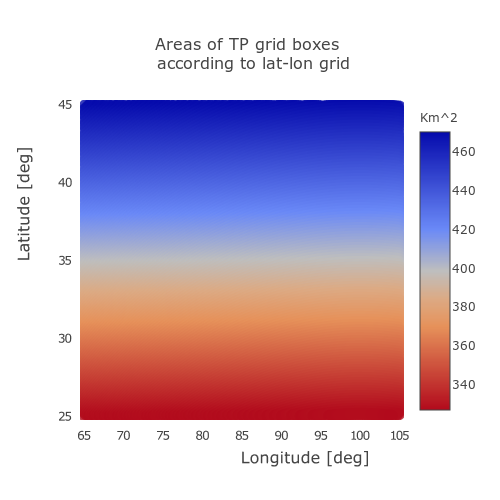
\includegraphics[width=\linewidth]{areas_of_tibet_grid_i.png}
\caption{\tiny{The area of a grid box varies according to latitude.}}
\end{minipage}
\end{figure}
\end{frame}

\begin{frame}
\frametitle{Calculating Areas: Estimate Grid Cell Area}
\begin{columns}
\column{0.450\textwidth}
\begin{figure}
\centering
\begin{minipage}{1\columnwidth}
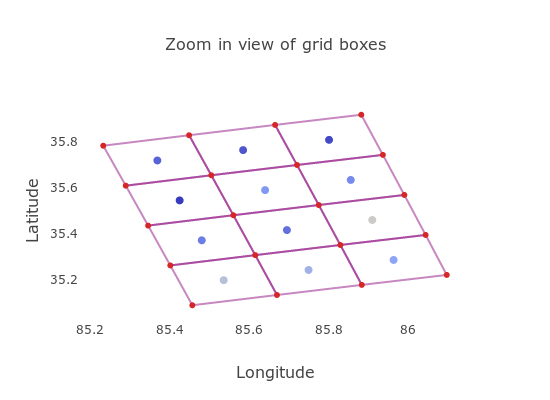
\includegraphics[width=\linewidth]{areas_of_subsection_i.png}
\caption{A zoom-in display of grid boxes and their centroid points provided a detailed view on how areas are estimated. Each central circle represents a lat-lon point provided by IMS. TSM calculates the red corner points followed by the bounding boxes' area.}
\end{minipage}
\end{figure}
\column{0.45\textwidth}
\begin{figure}
\centering
\begin{minipage}{1\columnwidth}
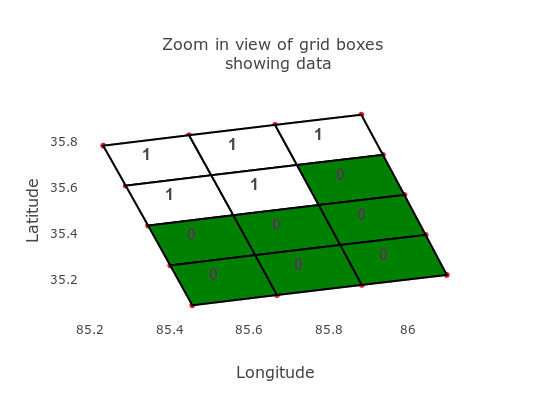
\includegraphics[width=\linewidth]{areas_of_subsection_ii.png}
\caption{A zoom-in view of the IMS data with snow/no snow illustrations. Cells covered in snow are in white and cells with no snow are shown in green.}
\end{minipage}
\end{figure}
\end{columns}
\end{frame}

\begin{frame}
\frametitle{Comparing LEAP Areas With Uniform Assumption}
\begin{figure}
\vspace*{-.5cm}
\centering
\begin{minipage}{.7\columnwidth}
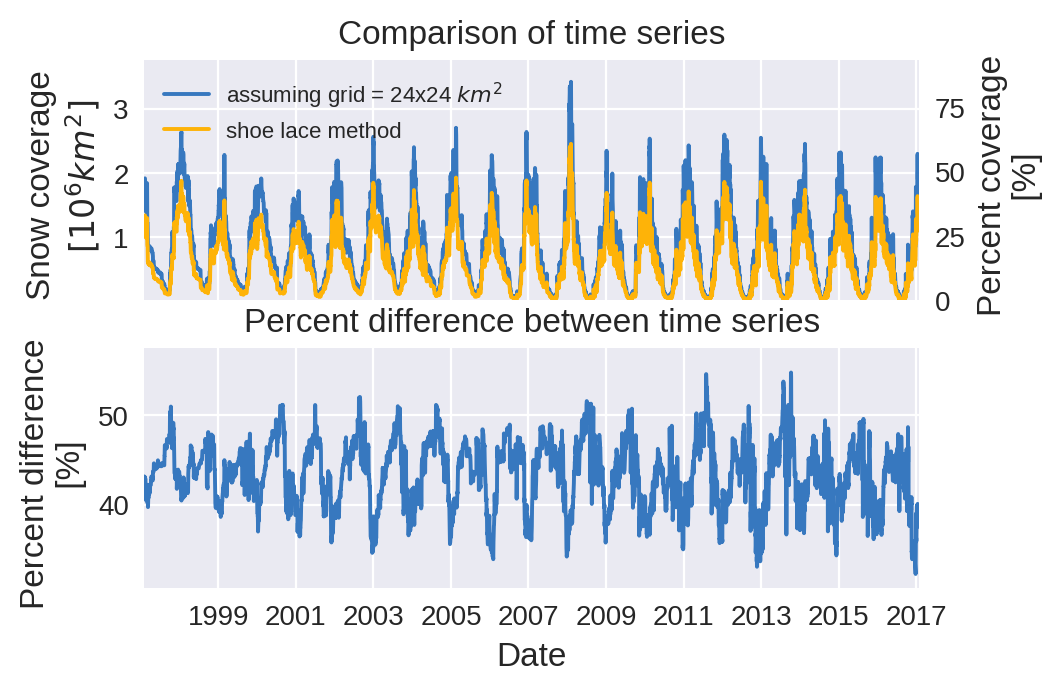
\includegraphics[width=\linewidth]{assumption.png}
\caption{Time series comparison between $24\times 24 km^{2}$ assumption and area calculation via shoe-lace formula.}
\end{minipage}
\end{figure}
\end{frame}

\begin{frame}
\frametitle{Comparing '$24km^{2}$' with  '$4km^{2}$' Resolutions}
\begin{figure}
\vspace*{-.5cm}
\centering
\begin{minipage}{.7\columnwidth}
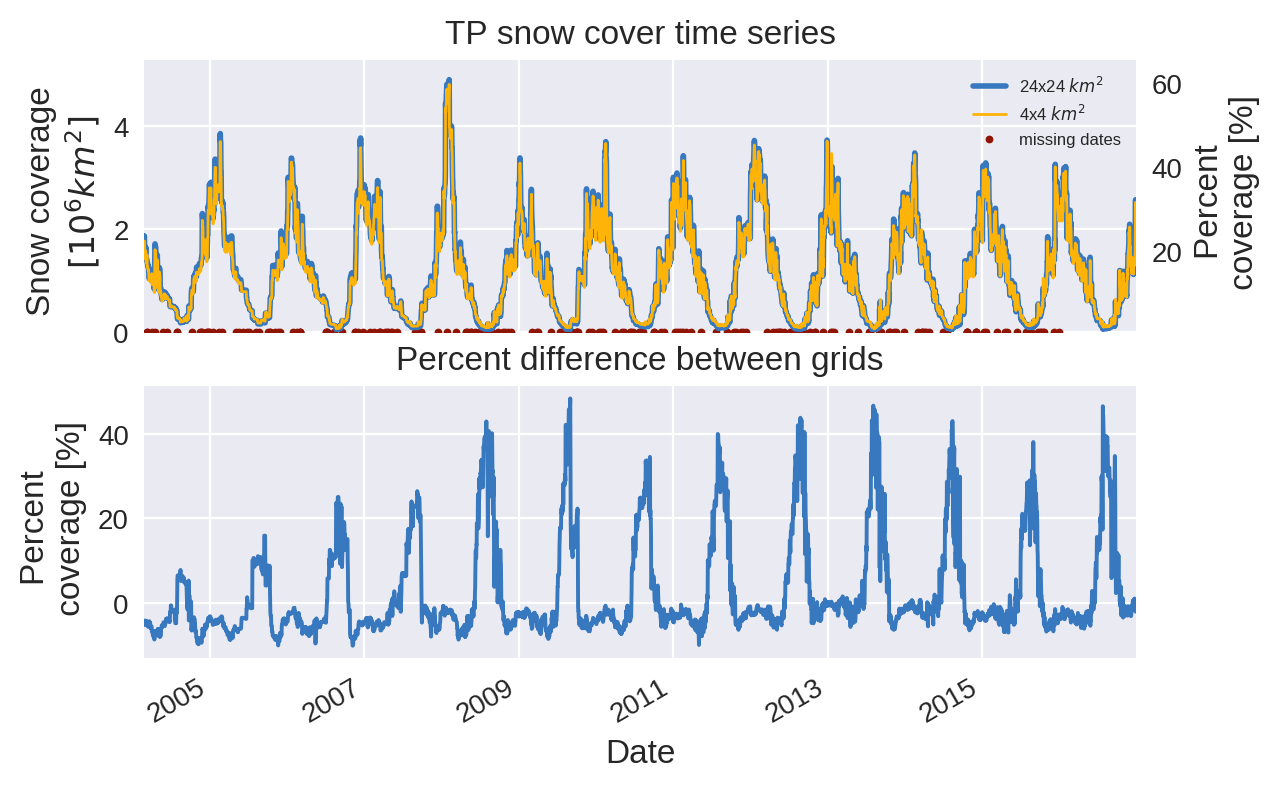
\includegraphics[width=\linewidth]{pres-24-4-compare.png}
\caption{The snow cover area time series comparison between two resolutions: 4 km and 24 km. Percent difference calculated using percent difference $100 * \left( \frac{ts_{24\ km} - ts_{4\ km}}{ts_{4\ km}} \right)$.}
\end{minipage}
\end{figure}
\end{frame}

\begin{frame}
\frametitle{Climatology: 5 Day Binning}
\begin{figure}
\centering
\begin{minipage}{.5\columnwidth}
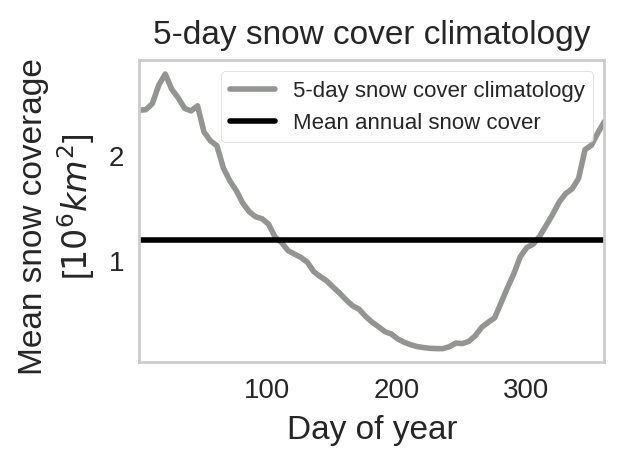
\includegraphics[width=\linewidth]{tibet-24-climate.png}
\caption{5 day climate averages of the $24 x 24$ km annual snow cycle.}
\end{minipage}
\end{figure}
\end{frame}

\begin{frame}
\frametitle{Climatology: STL via LOESS Regression}
\begin{columns}
\column{0.45\textwidth}
\begin{figure}
\centering
\begin{minipage}{1\columnwidth}
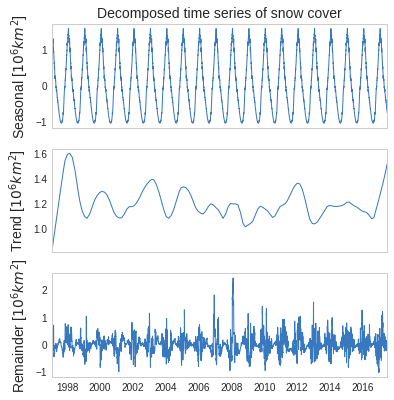
\includegraphics[width=\linewidth]{tibet-24-stl.png}
\caption{Deseasonalized using STL algorithm described in Appendex.}
\end{minipage}
\end{figure}
\column{0.45\textwidth}
\begin{block}{STL}
Seasonal Decomposition Based on LOESS by Cleveland et al 1990 allows a non stationary time series with a seasonal trend to be decomposed into three parts: The trend $T_t$, season $S_t$, and the residual $R_t$. Where the original signal $Z_t$ is combination of all three.
\begin{equation*}
Z_t = T_t + S_t + R_t
\end{equation*}
Implementation is done using the stl() function in R.
\end{block}
\end{columns}
\end{frame}

\begin{frame}
\frametitle{Anomalies}
\begin{columns}
\column{0.45\textwidth}
\begin{figure}[ht]
\centering
\begin{minipage}{1\columnwidth}
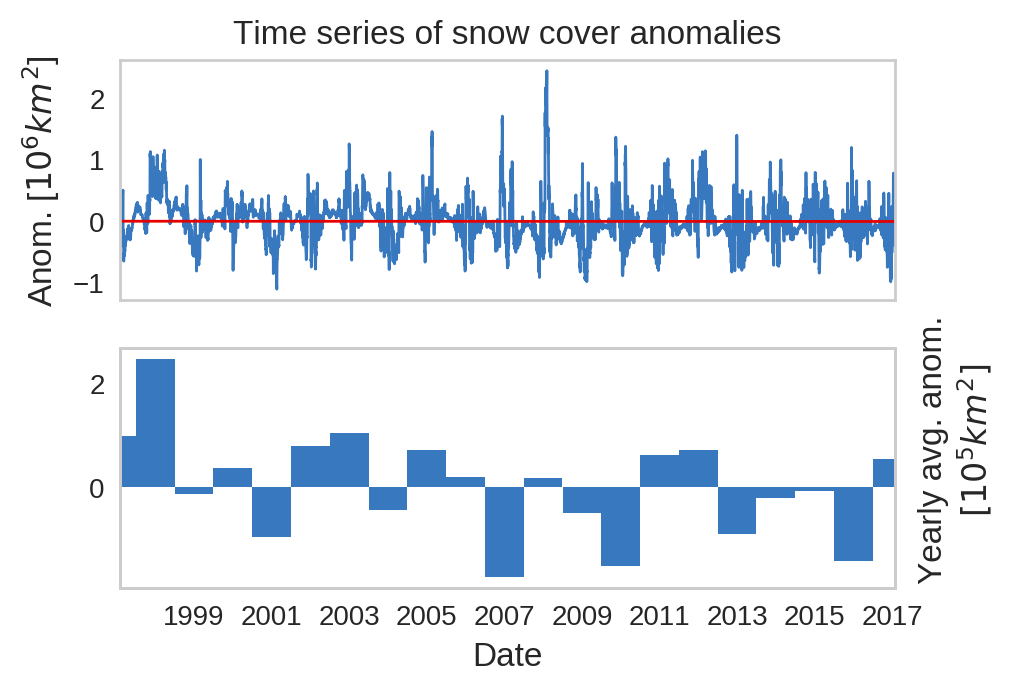
\includegraphics[width=\linewidth]{tibet-24-anomalies-ts.png}
\caption{Time series of Snow coverage anomalies with included trend line, in addition to yearly averaged anomalies, shown by the bar chart.}
\end{minipage}
\end{figure}
\column{0.45\textwidth}
\begin{block}{Anomalies}
5-day average climate model $clim(t)_{5}$ is subtracted from the time series, $Snow(t)$.
\begin{equation*}
Anomalies(t) = Snow(t)-clim(t)_{5}
\end{equation*}
Note that anomalies and STL remainder are attempting to deseasonalize the signal. Bother are not variance stationary.
\end{block}
\end{columns}
\end{frame}

\begin{frame}
\frametitle{Anomalies}
\begin{columns}
\column{0.30\textwidth}
\begin{table}
\centering
\caption{Anomaly Distribution Properties}
\hspace*{.5cm}\makebox[\linewidth][c]{%
\begin{tabular}{|c|c|}
\hline
\textbf{Statistic} & \textbf{Value}
\\ \hline
Mean\hphantom{00} & \hphantom{0}$-309.9 km^{2}$
\\ \hline
Median\hphantom{00} & \hphantom{0}$-30992 km^{2}$
\\ \hline
Min\hphantom{00} & \hphantom{0}$-1.112\ 10^6 km^{2}$
\\ \hline
Max\hphantom{00} & \hphantom{0}$2.446\ 10^6 km^{2}$
\\ \hline
Standard Deviation\hphantom{00} & \hphantom{0}$.34259971\ 10^6 km^{2}$
\\ \hline
Skew\hphantom{00} & $1.0006$
\\ \hline
Kurtosis (Pearson's) \hphantom{00} & $4.351$
\\ \hline
\end{tabular} }
\end{table}
\column{0.40\textwidth}
\begin{figure}
\hspace*{1cm}
\centering
\begin{minipage}{1\columnwidth}
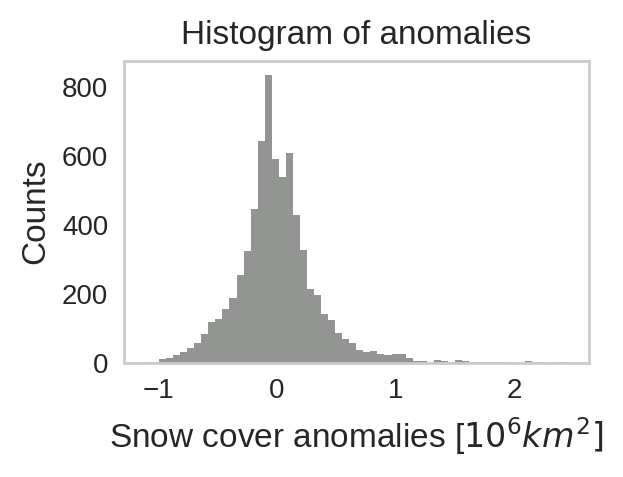
\includegraphics[width=\linewidth]{tibet-24-anomalies-hist.png}
\caption{Histogram of the $24 \times 24$ anomalies.}
\end{minipage}
\end{figure}
\end{columns}
\end{frame}

\begin{frame}
\frametitle{TSM as a Product}
\begin{columns}
\column{.45\columnwidth}
\begin{figure}
\vspace*{-1cm}
\centering
\begin{minipage}{1\columnwidth}
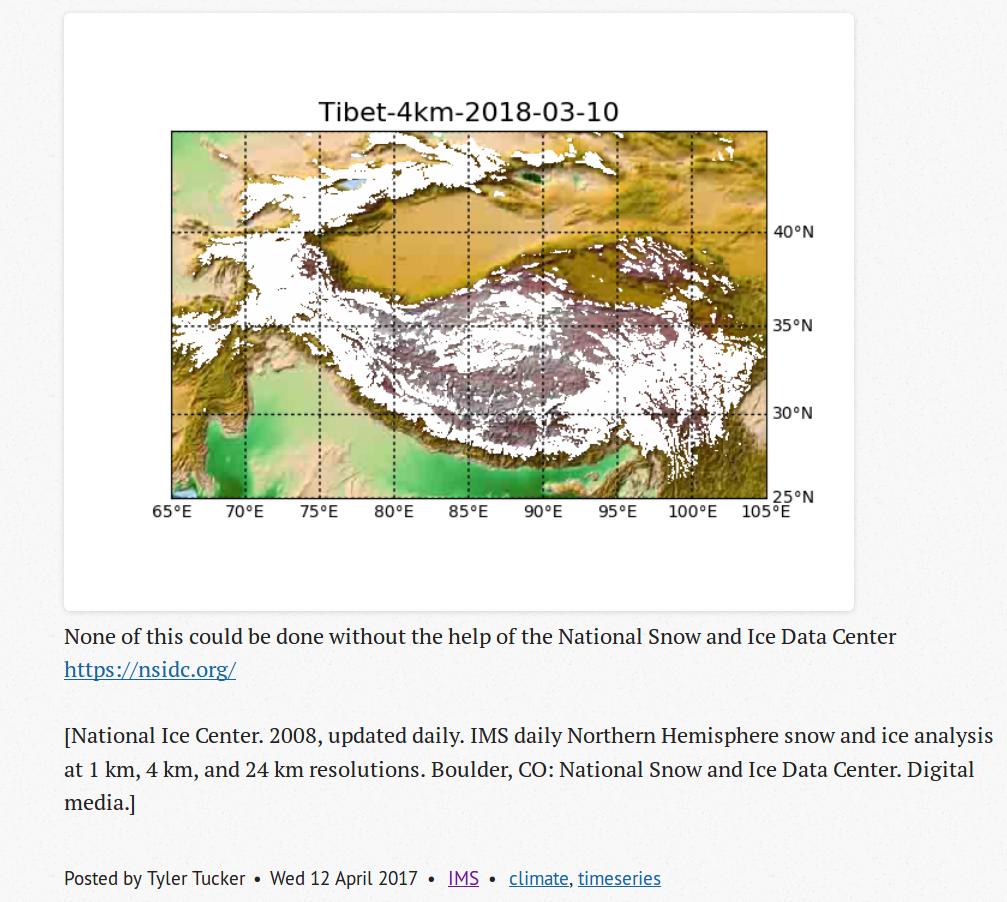
\includegraphics[width=\linewidth]{daily-tsm.png}
\caption{TSM is currently used to generate daily snow mapping at \url{http://www.itsonlyamodel.us/daily-snow.html}}
\end{minipage}
\end{figure}
\column{.45\columnwidth}
\begin{figure}
\vspace*{-.25cm}
\centering
\begin{minipage}{1\columnwidth}
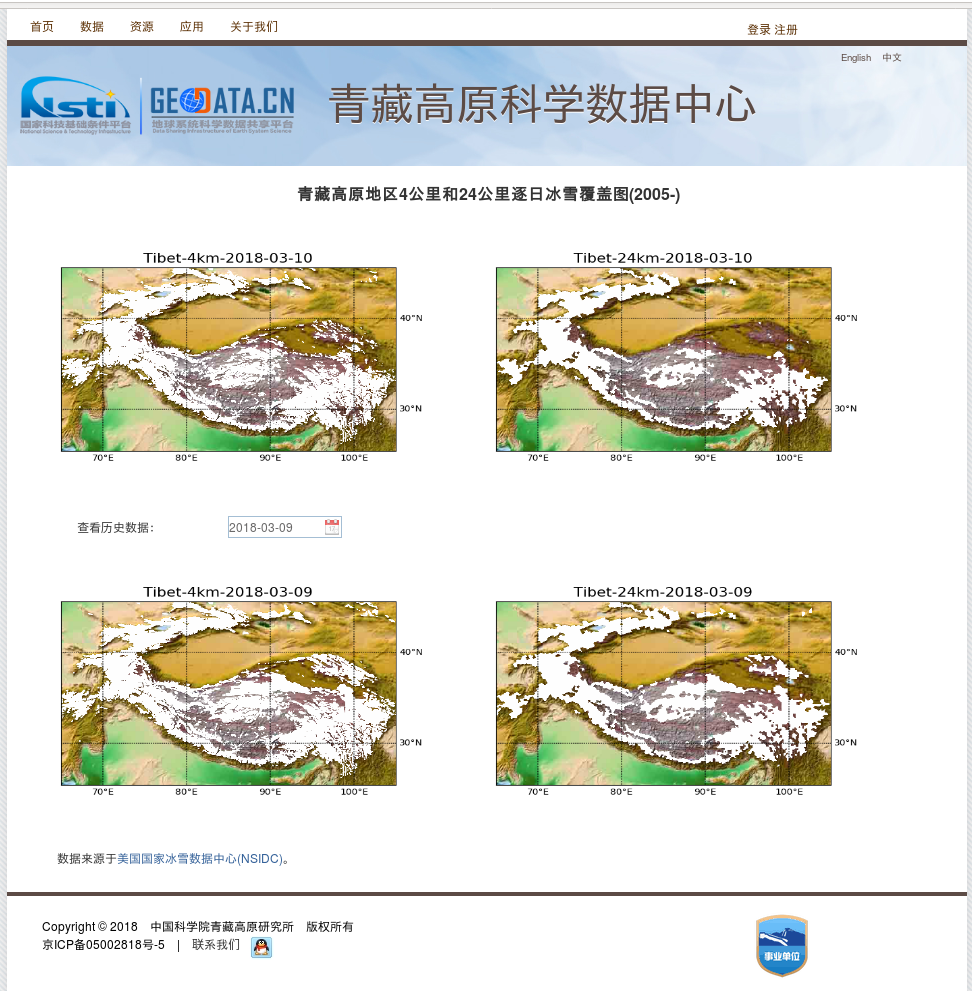
\includegraphics[width=\linewidth]{tpe-daily.png}
\caption{Screenshot of \url{http://www.tpedatabase.cn/tibetSnow.jsp} showing daily snow plot at archives at 24 and 4 km resolution.}
\end{minipage}
\end{figure}
\end{columns}
\end{frame}

\begin{frame}
\frametitle{TSM as a Product}
\begin{figure}
\vspace*{-1cm}
\centering
\begin{minipage}{1\columnwidth}
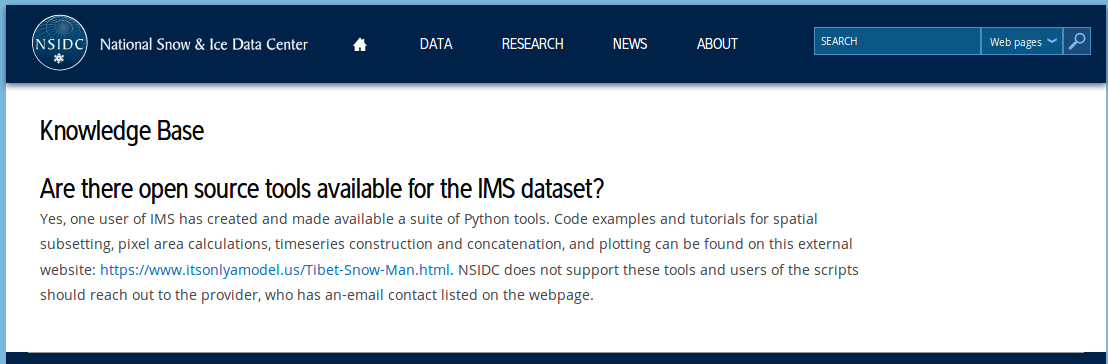
\includegraphics[width=\linewidth]{nsidc.png}
\caption{TSM is cited by NSIDC at at \url{http://nsidc.org/support/faq/are-there-open-source-tools-available-ims-dataset}}
\end{minipage}
\end{figure}
\end{frame}

\begin{frame}
\frametitle{Next Steps and Conclusion}
\begin{columns}
\column{0.45\textwidth}

\includegraphics[width=1\linewidth]{i-should-have-been-famous-a-minute-ago.jpg}
\column{0.45\textwidth}
\begin{itemize}
    \item Build code into a web app instead of a python library. Interactive web apps attract more users and researchers.
    \item IMS error is difficult to characterize. How can we estimate error, reduce bias? Can we trust these products?
    \item Apply this when they release a Southern Hemisphere Product
\end{itemize}
\end{columns}
\end{frame}